\chapter{Evaluation vorhandener Lösungsalternativen}
Im folgenden Kapitel werden drei Lösungsalternativen aus dem Google Play-Store zur Aufmaßerfassung vorgestellt und bewertet. Hierzu werden die benutzten Bewertungskriterien zunächst vorgestellt, und anschließend iterativ auf die ausgewählten Apps angewandt.

\section{Bewertungskriterien}
Zur Evaluation der Lösungsalternativen wird die erweiterte Version der Nielsen-Heuristiken \citep{Nielsen94}, sowie eine ausgewählte Menge selbst aufgestellter Kriterien benutzt.
Da sich die erweiterten Nielsen-Heuristiken aus 18 Kriterien zusammensetzen und nicht jede einzelne für die Bewertung der Lösungsalternativen gleich relevant ist bzw. sich nur bedingt anwenden lässt, werden die Kriterien klassifiziert (R = relevant, I = irrelavant).
Für die Evaluation der Apps werden anschließend nur Kriterien, die für eine mobile Android-Applikation zur Aufmaßerfassung im Gerüstbau relevant sind, benutzt.
\todo{Gewichtung überarbeiten}

\subsection{Die erweiterten Nielsen-Heuristiken}\label{subsec:nielsen}
 Nach \citeauthor{Nielsen94} gibt es zehn Heuristiken, die auf einer Grundlage von allgemein anerkannten Prinzipien beruhen, und sich zur Evaluation von Usability-Problemen besonders gut eignen \citep[Seiten 25--62]{Nielsen94}: 

\begin{enumerate}
    \di{Sichtbarkeit des Systemzustandes (R)}{N1}{Angemessene Rückmeldung in einem vernünftigen zeitlichen Rahmen}
    \di{Übereinstimmung zwischen System und realer Welt (I)}{N2}{Sprache des Benutzers, natürliche und logische Reihenfolge}
    \di{Benutzerkontrolle und -freiheit (R)}{N3}{Undo und Redo}
    \di{Konsistenz und Standards (R)}{N4}{Konsistente Nutzung und Beachtung der Plattform-Konventionen}
    \di{Fehlervorbeugung (R)}{N5}{Vermeide Situationen in denen Fehler entstehen können}
    \di{Wiedererkennung statt Erinnern (R)}{N6}{Objekte, Optionen und Aktionen sollen sichtbar sein}
    \di{Flexibilität und Effizienz der Benutzung (R)}{N7}{Häufige Aktionen anpassbar, Experten schnellere Bedienung erlauben}
    \di{Ästethisches und minimalistisches Design (R)}{N8}{Keine irrelevanten Informationen}
    \di{Erkennbarkeit, Diagnose und Erholung von Fehlern (I)}{N9}{Verständliche Fehlermeldungen}
    \di{Hilfe und Dokumentation (1)}{N10}{Leicht zu finden, abgestimmt auf Aufgabe, konkrete Schritte zur Lösung}
\end{enumerate} 

\noindent
Zur Bewertung von Software auf mobilen Endgeräten reichen diese zehn Bewertungskriterien jedoch nicht vollständig aus, sodass weitere acht Heuristiken, die speziell für mobile Geräte ausgelegt sind, hizugezogen werden \todo{ref auf ue, 239}:

\begin{enumerate}
	  \setcounter{enumi}{10}
    \di{Adäquater Umgang mit Unterbrechnungen (R)}{N11}{Kein Verlust von Informationen bei Unterbrechung der Aktivität}
    \di{Fokussieren der Informationen (I)}{N12}{Hervorheben der wichtigen Informationen, um schnelles Scannen zu erlauben}
    \di{``Joy of Use'' (R)}{N13}{Positives Nutzungserlebnis bei Bedienung/Verwendung}
    \di{``Don't lie to the user'' (I)}{N14}{Keine falschen oder ungültigen Zahlen, Fakten bzw. Nachrichten}
    \di{Unterstützung verschiedener Bildschirmausrichtungen (R)}{N15}{Keine Verwirrung bei verschiedenen Ausrichtungen des Bildschirms}
    \di{Ergonomische Gestaltung der physischen Interatkion (Rj}{N16}{Kein unabsichtliches Auslösen von Funktionen}
    \di{Einfache Eingabe, Bildschirmlesbarkeit und Übersichtlichkeit (R)}{N17}{Einfache Navigations- und Eingabetechniken bei einhändiger Benutzung}
    \di{Stelle Privatheit sicher (R)}{N18}{Vermeide den Verlust/Diebstahl von privaten Daten z.b. durch Passwörter}
\end{enumerate}

\subsection{Weitere Kriterien}
Zusätzlich zu den in \autoref{subsec:nielsen} vorgestellen Heuristiken werden noch zwei weitere Kriterien zur Evaluation hinzugezogen, die für die Benutzung der App aus Sicht der Aufmaßerfassung im Gerüstbau wichtig sind: \todo{anders formulieren}

\begin{itemize}
    \di{Integration der App in eine vorhandene Systemarchitektur}{integration}{Die Software-Lösung sollte sich in eine bereits vorhandene Systemarchitektur integrieren lassen}
    \di{Export des annotierten Bildes und der Metadaten zur Weiterverarbeitung in einem nachgelagerten Dienst (z.B. API)}{export}{Die App sollte die eingetragenen Meta-Daten, wie zum Beispiel die Längen einer Linie, zur Weiterverarbeitung exportierbar machen}
	  \todo{mehr Kriterien raussuchen}
\end{itemize}

\section{Vorstellung und Evalutation ausgewählter Apps}
Als Lösungsalternativen wurden drei Android-Applikationen, die unter dem Suchbegriff ``Aufmaße'' im Google Play-Store verfügbar sind, ausgewählt.
Hierbei handelt es sich um folgende drei Apps:

\begin{itemize}
  \item \mm{} - Bosch GmbH
  \item \ms{} - SameBits
  \item \pm{} - Blue Big Pixel Inc.
\end{itemize}

\noindent
\todo{Quellen} 
Es wurden gerade diese Apps zur Evalutation ausgewählt, da sie verschiedene Auswahlkriterien verschienden stark ausfüllen.
So stammt die App \mm{} von einem großen Unternehmen mit mehr als 80 Standorten in Deutschland, und einem Jahresumsatz von 14,5 Mrd. Euro. \\
\ms{} wurde gewählt, da sie mit 100.000 bis 500.000 Installationen eine der populärsten Apps unter dem Suchbegriff ``Aufmaße '' ist. \\
Im Gegensatz dazu verzeichnet \pm{} bei einem Zehntel der Installation eine durschnittliche Bewertung von 4,3 von 5 Sternen im Google Play-Store, was sie damit zu einer der beliebtesten Apps unter dem Suchbegriff ``Aufmaße'' macht.

\subsection{Measuring Master}

\subsubsection{Vorstellung}
\todo{Version, Downloaddatum, Playstore-Link}
Die App \mm{} von der Bosch GmbH ist im Play-Store unter der Rubrik ``Effizienz'' aufgelistet.
Selbst beschreibt der App-Hersteller seine Software wie folgt \citep{BoschMM}:

\begin{quote}
  ``Measuring Master ist eine multifunktionale App, die es ermöglicht, Aufmaße, Grundrisse und Temperaturmesswerte an einem Ort zu dokumentieren und zu verwalten.\\
  Die App ist besonders geeignet für Architekten, Maler, Bodenleger, Heizungsbauer und Elektriker, aber auch alle anderen Handwerker profitieren von der umfangreichen Funktionalität''
\end{quote}

\noindent
Nach dem Start der Applikation bietet sich die Möglichkeit ein neues Projekt anzulegen, oder bereits vorhandene Projekte zu bearbeiten.
Sobald das gewünschte Projekt ausgewählt wurde, bieten sich dem Benutzer über das Menü an der linken Seite diverse Funktionen (siehe \autoref{fig:bmenu}) an. \\

\begin{figure}[h]
  \centering
	\begin{subfigure}[t]{0.4\textwidth}
		\includegraphics[keepaspectratio, width=\textwidth]{bosch/menu}
		\caption{Navigationsmenü}
		\label{fig:bmenu}	
	\end{subfigure}
	\begin{subfigure}[t]{0.4\textwidth}
		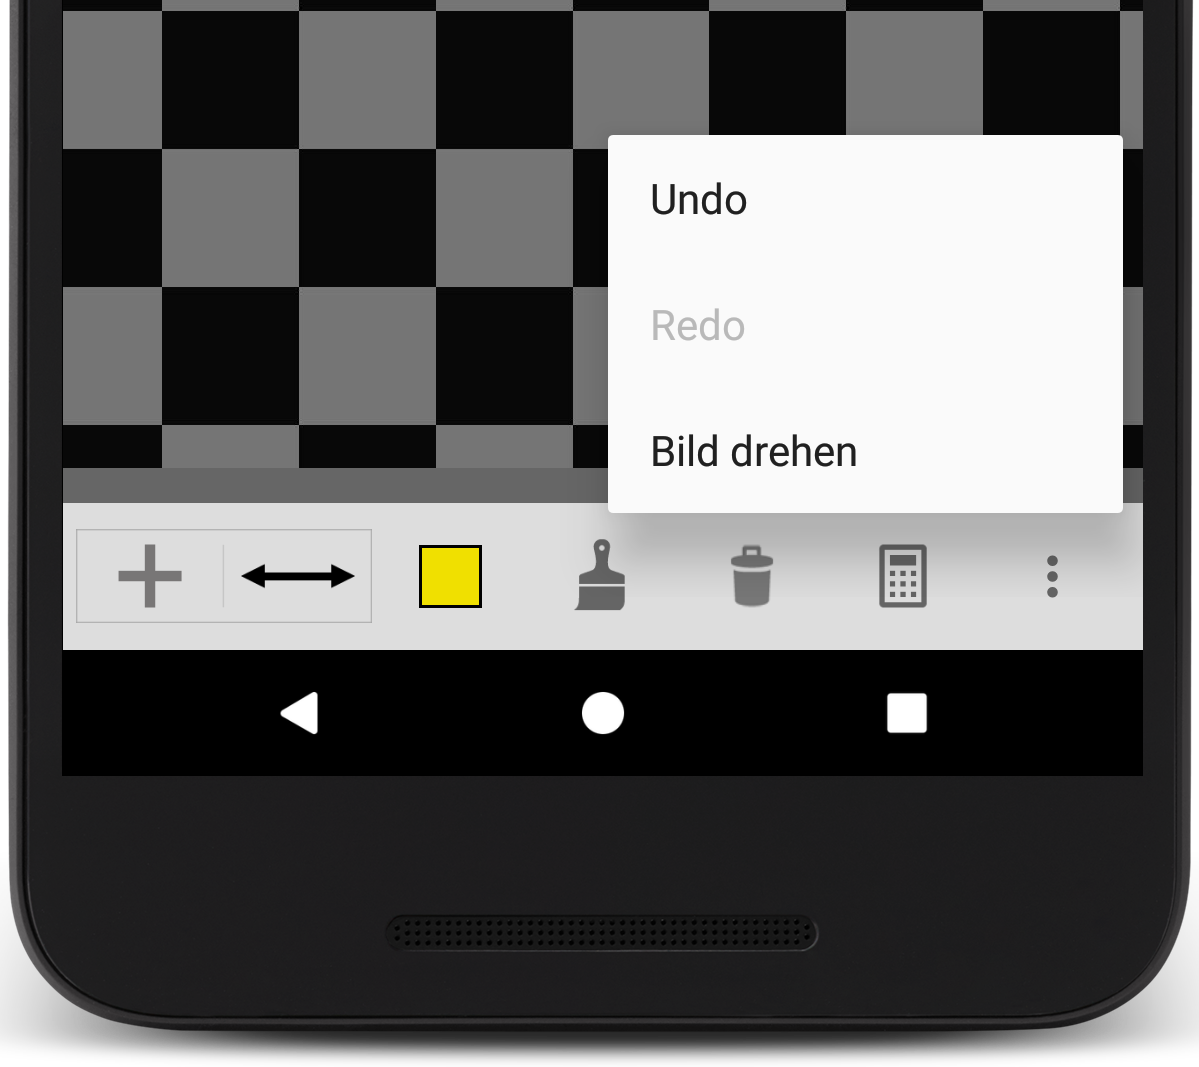
\includegraphics[keepaspectratio, width=\textwidth]{bosch/bar}
		\caption{Aufmaße-Funktion}
		\label{fig:bbar}	
	\end{subfigure}
  \caption{\mm{} bei ausgeklapptem Navigationsmenü und in der Aufmaße-Funktion}
\end{figure}

Im Folgenden wird der Menüpunkt ``Aufmaße'' und die damit verbundene Funktionalität weiter vorgestellt und evaluiert.
So bietet sich dem Benutzer nach Auswahl der Aufmaße-Funktion die Möglichkeit, ausgewählte Bilder direkt mit Messwerten zu beschriften.
Hierzu können entweder Bilder direkt aus der Gallerie importiert, oder mit der Kamera aufgenommen werden.
Sobald der Benutzer den Foto-Import erfolgreich abgeschlossen hat, öffnet sich eine neue Ansicht, welche das ausgewählte Bild und weitere Bedienelement, in Form einer Statusleiste am unteren Rand, zeigt (siehe \autoref{fig:bbar}). \\

In dieser Benutzeroberfläche kann der Nutzer mit Hilfe von vier verschiedenen Formen (Linie, Viereck, Winkel, Freiform) Aufmaße ins Bild anzeichnen, und über einen Klick auf die gewünschte Form, Messwerte eintragen.
Außerdem bietet die App die Option, eine ausgewählte Reihe von Laserentfernungsmesser mit der App zu verbinden.
Dies ermöglicht eine Übertraung der gemessenen Distanzen über eine Bluetooth-Schnittstelle direkt an die App. \\

Um das annotierte Bild außerhalb der App weiter zu benutzen, bietet diese den Export als \emph{PDF} und \emph{JPEG} an.
Die exportierte \emph{PDF} enthält im Gegensatz zu der \emph{JPEG} zusätzlich zu dem annotierten Bild auch noch eine Tabelle mit allen eingetragenen Messwerten \autoref{fig:bexport}. 
Zudem lassen sich annotierte Bilder in der App speichern und zu einem späteren Zeitpunkt wieder bearbeiten.

\begin{figure}[h]
  \centering
  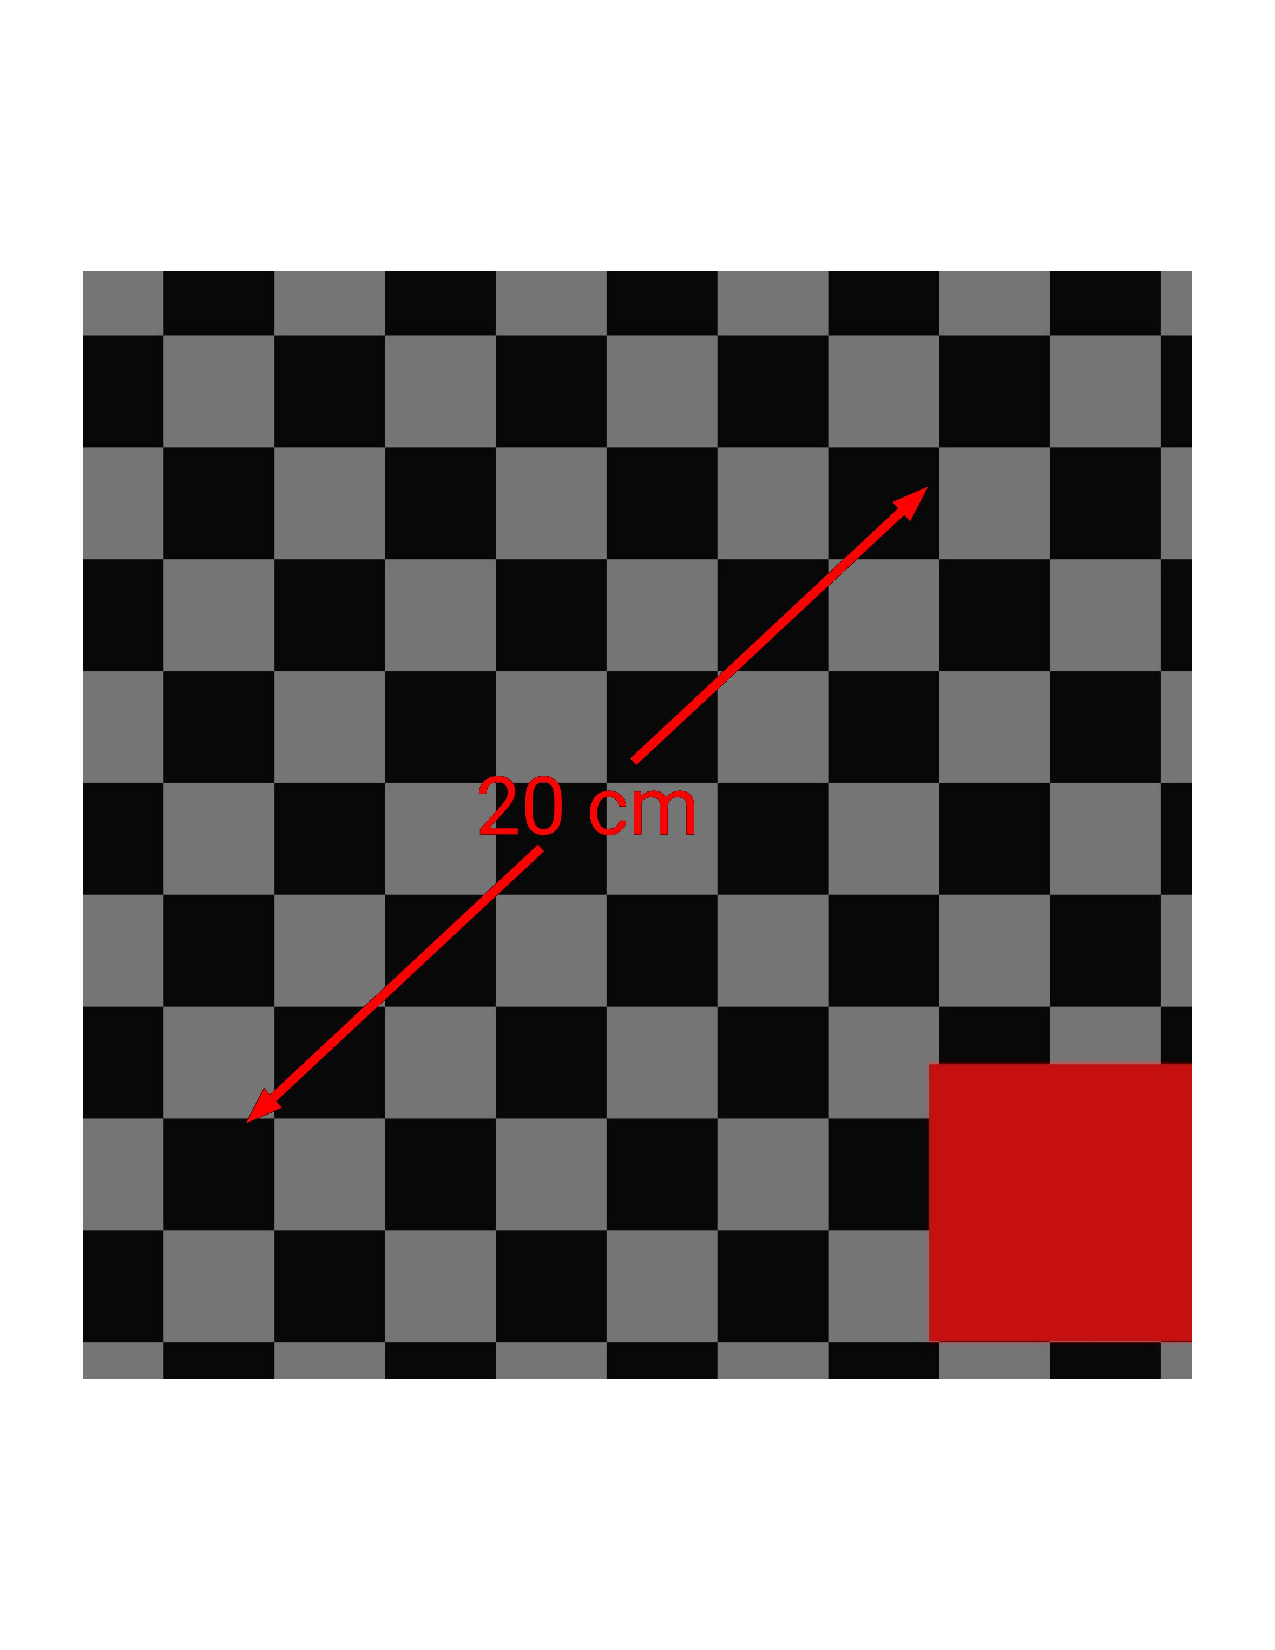
\includegraphics[keepaspectratio, width=\textwidth]{bosch/export}
  \caption{Exportierte PDF}
  \label{fig:bexport}
\end{figure}

\subsubsection{Evaluation}

Die App zeigt in einer Art Statusleiste am unteren Rand des Bildschirms den aktuellen Modus an, und gibt über einen auffordernden Text am oberen Bildschirmrand dem Nutzer eine Hilfestellung, was er im gerade ausgewählten Modus machen kann. \todo{screens} Hiermit deckt die App Nielsen \ref{itm:1} und \ref{itm:10} ausreichend ab. \\

Des Weiteren benutzt auch diese App universell verständliche Icons, um die wichtigsten Aktionen wiedererkennbar zu machen. So hat beispielsweise das Mülleimer-Icon in jedem Modus die Löschfunktion. \\

Im Gegensatz zu \textsc{Photo Measures} bietet diese App dem Benutzer die Möglichkeit seine Aktionen rückgängig zu machen, oder sie zu wiederholen. Dies ist ein deutlicher Vorteil seitens der Usability, da Fehler nicht so hart bestraft werden, als wenn keine Undo/Redo-Button vorhanden wären. \\

Fehler werden hier durch das Deaktivieren von Buttons, die im aktuellen Systemzustand nicht benutzbar sind, präventiv verhindert. Das Löschen von Formen ist beispielsweise nur dann möglich, wenn zuvor eine Form ausgewählt wurde.

Negativ fällt auch in dieser Alternative die fehlerhafte Gesten-Unterstützung auf. So sorgen Zoom-Gesten per Doppel-Tap zum unabsichtlichen Zeichnen einer Form, welche im Nachhinein wieder gelöscht werden muss. Außerdem verletzt die App Nielsen~\ref{itm:15}, da Änderungen in der Bildschirmausrichtung dafür sorgen, dass das Bild nicht wie erwartet seine Ursprungsausrichtung beibehält, sonder auch rotiert wird. 

\subsection{Measure \& Sketch}
\subsubsection{Vorstellung}
Die App \emph{Measure \& Sketch} wird von \emph{SameBits} entwickelt.
Zur Zeit des Downloads (20. Januar 2018) ist die Applikation laut Google Play-Store auf zwischen $100.000$ und $500.000$ Android-Geräten installiert.
Auch diese Applikation ist unter der Kategorie ``Effizienz'' gelistet, und wird vom Entwickler mit den folgenden Worten beschrieben \citep{BitsMS}:

\begin{quote}
  ``Die Must-Have Zeichenapp für alle echten Ingenieure, Architekten, Bauarbeiter, Immobilienmakler, Handwerker wund [sic] natürlich für alle Heimwerker!''
\end{quote}

\noindent
Beim initialen Start der App wird der Benutzer mit Hilfe eines Overlays auf die möglichen Aktionen, die er in diesem Zustand tätigen kann, hingewiesen.
Hier bietet sich die Option zwischen den bestehenden Projekten zu wechseln, oder ein Neues anzulegen.
Über den Knopf ``Neu'' (siehe \autoref{fig:msmenu} kann der Nutzer ein neues Bild aufnehmen, oder direkt eines aus der Galerie importieren. \\

\begin{figure}[h]
  \centering
	\begin{subfigure}[t]{0.4\textwidth}
		\includegraphics[keepaspectratio, width=\textwidth]{measure_sketch/menu}
		\caption{Startbildschirm}
		\label{fig:msmenu}	
	\end{subfigure}
	\begin{subfigure}[t]{0.4\textwidth}
		\includegraphics[keepaspectratio, width=\textwidth]{measure_sketch/menu}
		\caption{Aufmaße-Funktion} 
		\label{fig:msbar}	
	\end{subfigure}
  \caption{Measure \& Sketch beim Start der App und in der Aufmaße-Funktion}
\end{figure}

\noindent
\todo{Bilder mit Overlay}
Sobald man ein Bild ausgewählt hat, öffnet sich eine neue Benutzeröberfläche, in der, wie schon beim Start der App, durch ein Overlay alle möglichen Aktionen beschrieben werden (siehe \autoref{fig:msbar}).
In dieser Ansicht kann man das Bild mit drei verschiedenen Formen (Linie, Winkel, Freitext) annotieren. 
Zusätzlich können eingezeichnete Formen mit Messwerten beschriftet werden.\\

Weiterhin bietet sich die Gelegenheit, das bearbeitete Bild zur Galerie, \emph{Evernote} oder Universal \todo{gucken was gemeint ist} zu exportieren, oder direkt per E-Mail zu verschicken.
Auch bei dieser App kann man modifizierte Bilder speichern, und zu einem späteren Zeitpunkt zur Weiterverarbeitung wieder öffnen. \\

\subsubsection{Evaluation}

\begin{wrapfigure}{R}{0.4\textwidth}
	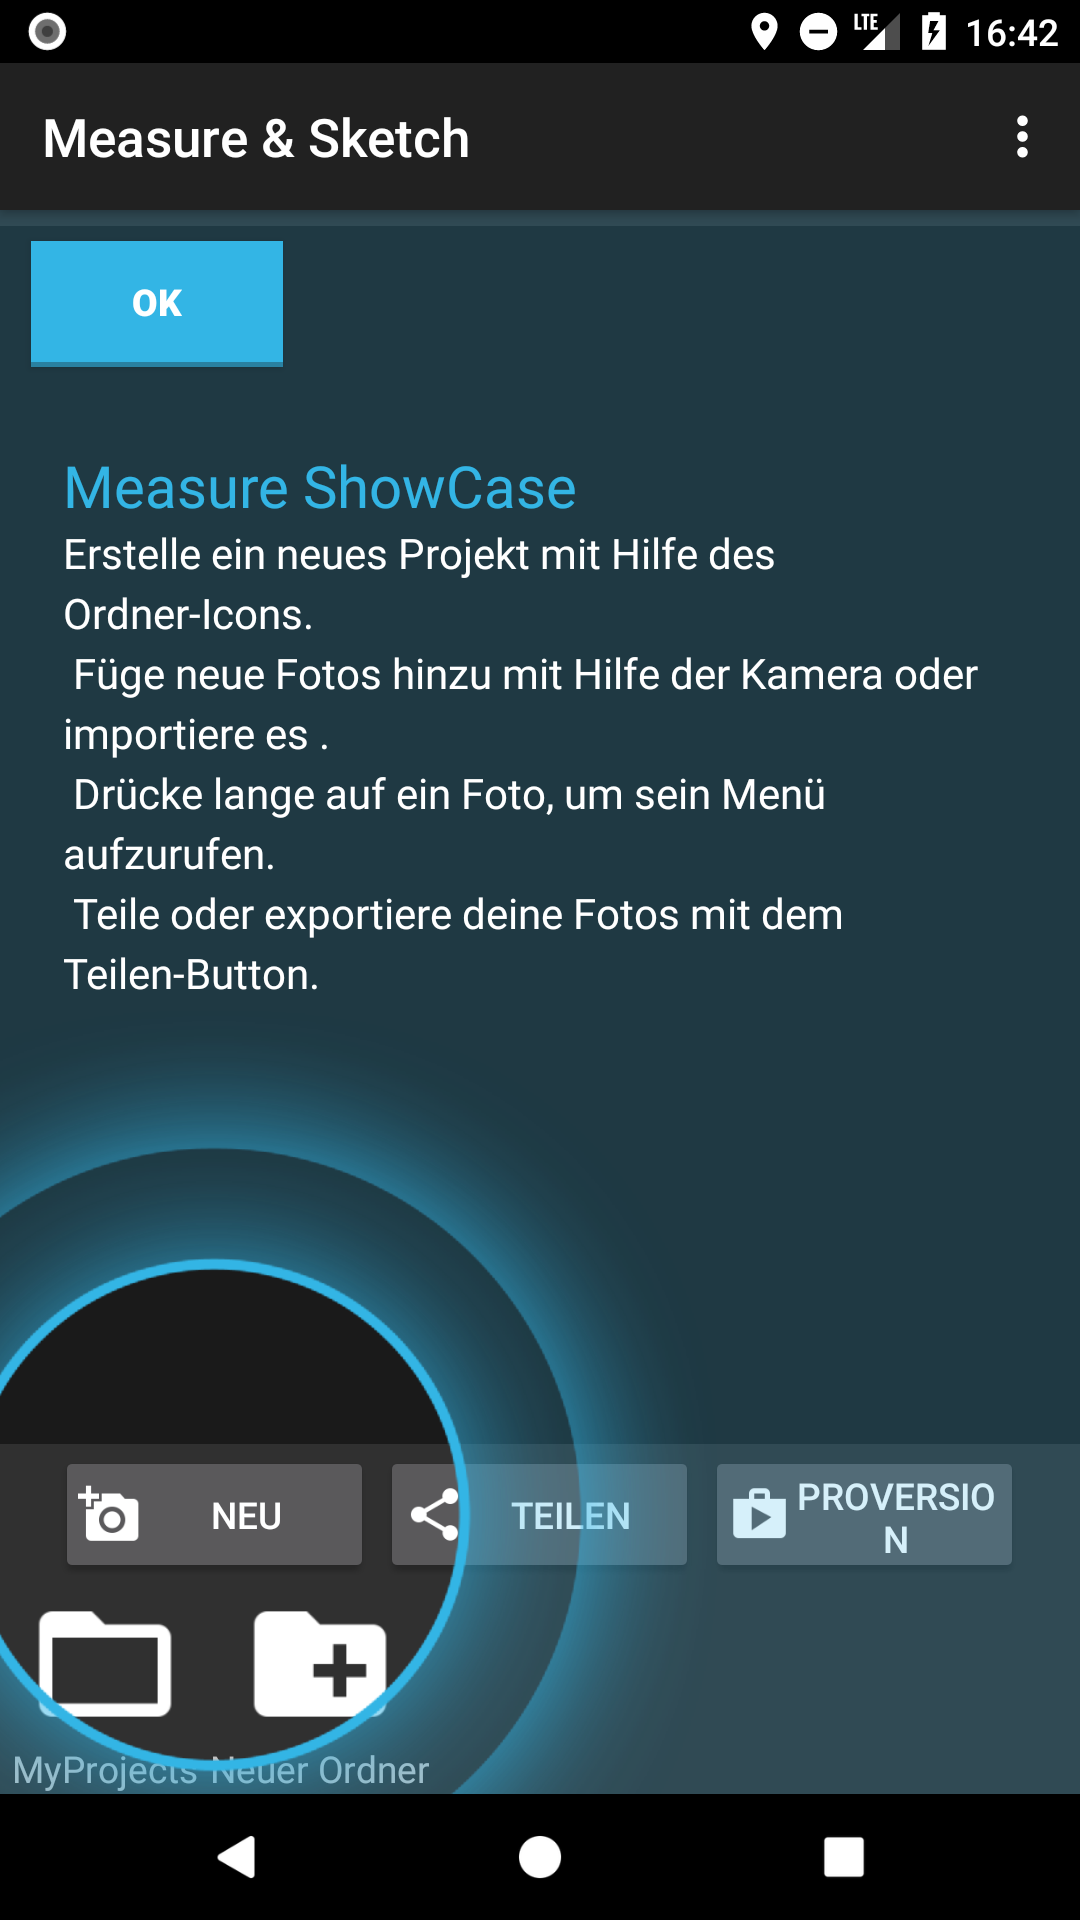
\includegraphics[keepaspectratio, width=0.4\textwidth]{measure_sketch/help_start}
	\caption{Hilfe-Overlay}
	\label{fig:mshelp}
\end{wrapfigure}

Auch diese App bedient sich eines Hilfe-Overlays beim ersten Start, überfordert den Benutzer jedoch mit zu viel Text. So erfüllt dieses Tooltip ihre Funktion als Hilfestellung nicht, sondern überfordert den Nutzer mit Text. Alternativ bietet sich auch bei dieser App wie in \autoref{fig:pmhelp} mit Icons zu arbeiten, sodass die Gedächtnisbelastung minimiert wird. \\

Die App kann als negativ-Beispiel bezüglich der Nielsen-Heuristiken betrachtet werden. Es gibt weder Undo- oder Redo-Button, noch wird in irgendeiner Weise hervorgehoben, welche Form aktuell ausgewählt ist. Dies führte beim Löschen oft zu Überraschungen. \\

 Außerdem unterstützt die App keinerlei Gesten zur Navigation im Bild. So lässt sich der abgebildete Bereich des Bildes weder zoomen, noch kann der Benutzer das Bild rotieren oder verschieben. Um Formen zu zeichnen bedient sich die App eine für den Benutzer unnatürliche Geste, denn hierzu muss der Nutzer gleichzeitig mit zwei Fingern die Form in die beiden gewünschten Richtungen ``aufziehen''. So fühlt sich der Zeichen-Prozess nicht nur unnatürlich an, sondern ist in der Größe der Form durch die Spannweite der Finger des Benutzers beschränkt. \\
 
 Zusätzlich schließt dies die Benutzung der App mit einer Hand aus, was Nielsen~\autoref{itm:16} klar widerspricht. Als Bildschirmausrichtung wird nur der Portrait-Modus unterstützt, was gerade die Bearbeitung von im Landscape aufgenommenen Bildern zu einer Herausforderung macht. \\


\subsection{Photo Measures}
hallo


\section{Auswertung der Evaluationsergebnisse}
Fazit und Überleitung zur Konzeption eigener App
